\chapter{Introduction}
\label{ch:introduction}
\section{Problem Description}
In recent years, the way people purchase and manage clothing has been significantly influenced by the growth of online shopping. Users can choose from a wide range of clothing options, and many applications try to help with different parts of the dressing process.

Despite these developments, making daily outfit decisions remains a challenge in practice. Users often find it difficult to imagine how clothes would look on themselves, efficiently organize their existing wardrobe, and choose appropriate outfits for different occasions. These challenges highlight the need for more effective tools to support users' overall decision-making process.

\subsection{Existing Market Applications}
\label{chapter: Existing Market Applications}
As shown in Figure \ref{fig:app-comparison}, existing wardrobe-related applications have already provided partial support for users during different stages of the dressing process. Virtual try-on tools such as \textbf{Fitle} and \textbf{AI Try-On} reduce uncertainty in online shopping by offering visual simulations of clothing on the human body. Meanwhile, digital wardrobe systems like \textbf{Whering} and \textbf{Smart Closet} allow users to organize their clothing, manage items, and plan outfits.

\noindent\textbf{Clarification for Figure~\ref{fig:app-comparison} below:}
\begin{itemize}
    \item \textbf{Platform:} \textbf{G} represents Google Play, and \textbf{A} represents the App Store.
    \item \textbf{Devices:} 
    \begin{itemize}
        \item \textbf{3} indicates iPhone, iPad, and Mac;
        \item \textbf{2} indicates iPhone and iPad;
        \item \textbf{1} indicates iPhone only.
    \end{itemize}
\end{itemize}

\begin{figure}[H]
    \centering
    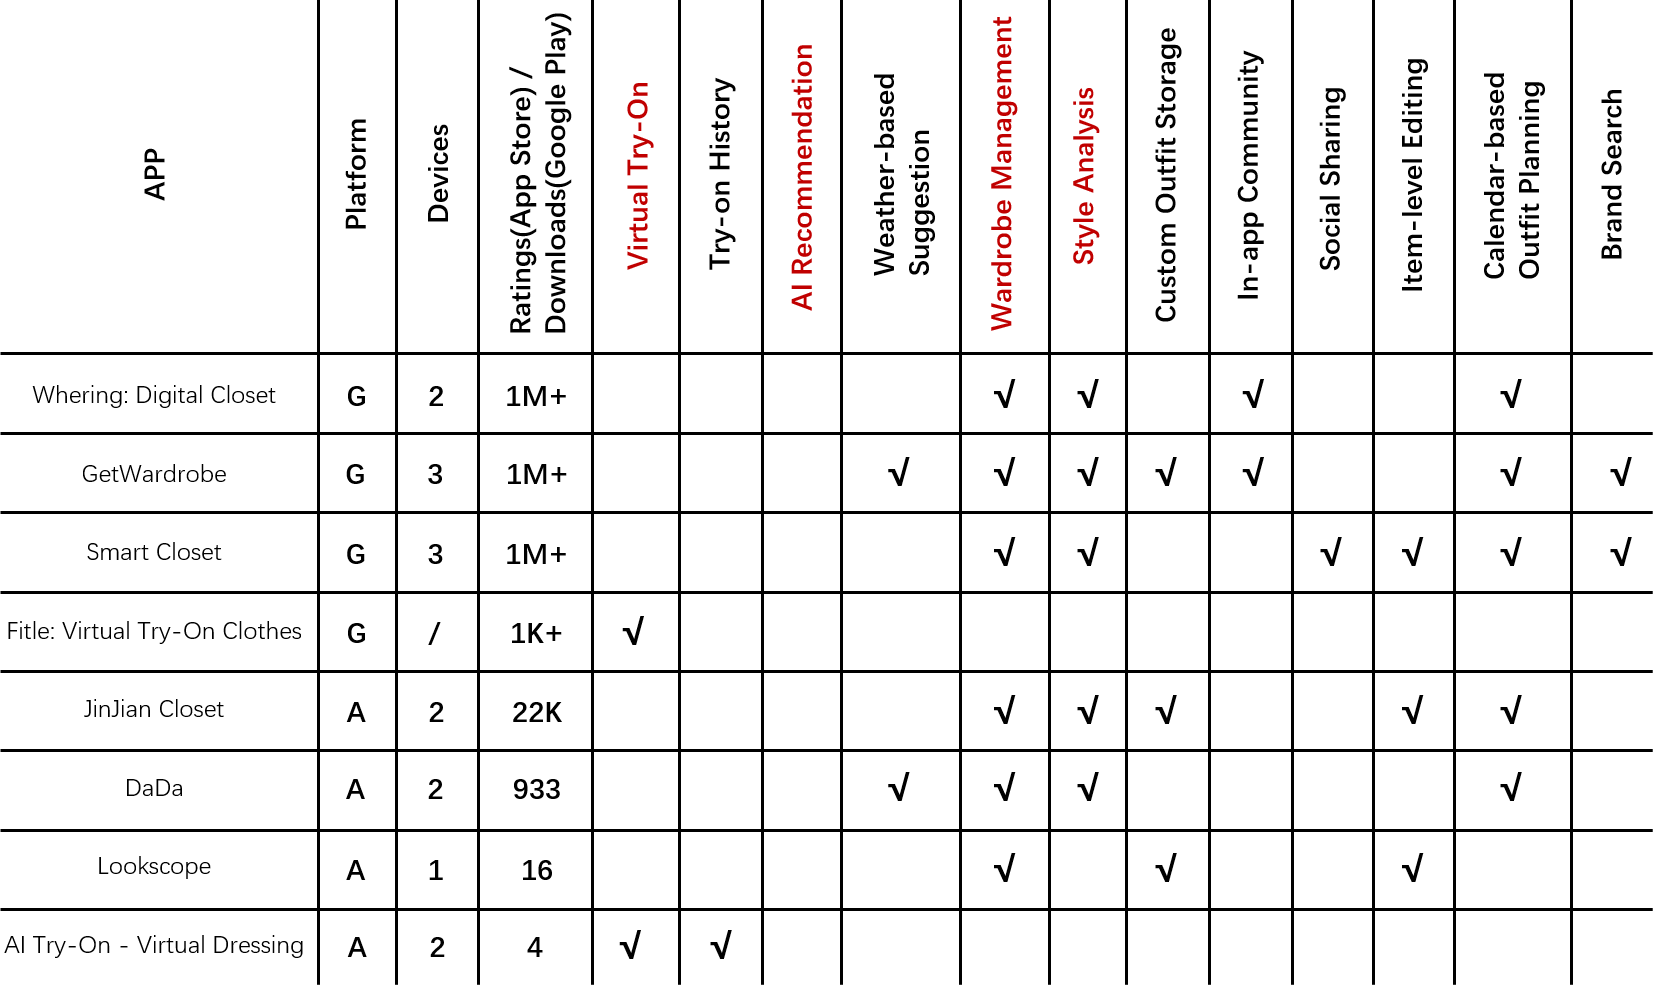
\includegraphics[width=1.0\textwidth]{images/Section_2_industryBackground/app.png}
    \caption{Existing Applications}
    \label{fig:app-comparison}
\end{figure}


However, these applications remain functionally fragmented. Those with virtual try-on capabilities typically provide only image-based visualization and are not connected to the user's personal wardrobes or preferences. Therefore, the try-on results cannot directly assist users in making outfit decisions.


\begin{figure}[H]
    \centering
    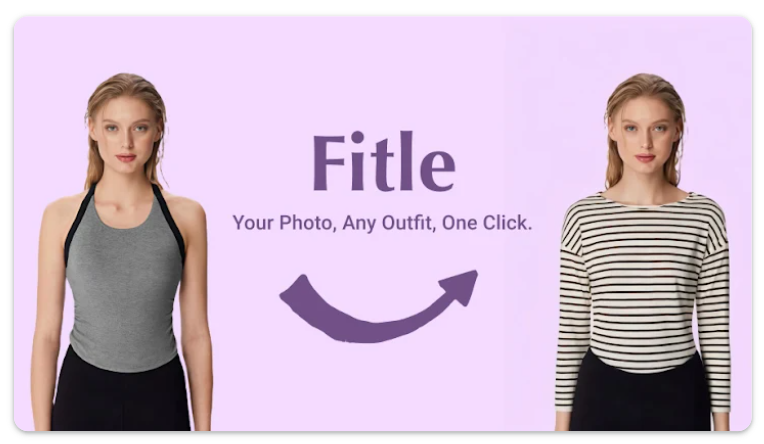
\includegraphics[width=0.7\textwidth]{images/Section_2_industryBackground/Fitle.png}
    \hfill
    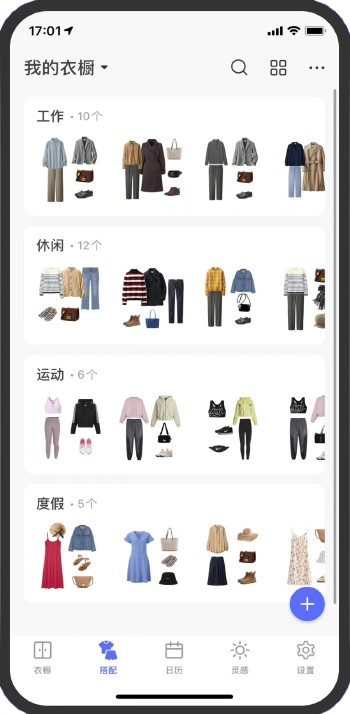
\includegraphics[width=0.25\textwidth]{images/Section_2_industryBackground/JinJian.jpg}
    \caption{Virtual Try-on in Fitle (left, \citep{Fitle_closet_appstore}) and Wardrobe Management in JinJian (right, \citep{JianJin_closet_appstore})}
    \label{fig:app}
\end{figure}

On the other hand, wardrobe management applications such as \textbf{Smart Closet} and \textbf{JinJian Closet} (Fig.~\ref{fig:app}) are relatively mature in item organization, but they largely rely on manual operations. They lack semantic understanding and the ability to automatically generate tags or outfits, which limits their capability to ease the user's dressing decision burden.


Some applications, such as \textbf{GetWardrobe} and \textbf{DaDa}, provide weather-based suggestions. However, these recommendations usually only take into account simple temperature, without considering the activity occasions or personal preferences, making them less practical in actual use.


\subsection{Gap Analysis}
Based on the analysis of existing applications, the main limitation lies in the lack of functional integration. Most systems only focus on a single aspect, such as virtual try-on, wardrobe management, or basic recommendation, but fail to combine these functionalities into a complete workflow.

Furthermore, current recommendation systems tend to be overly general and lack explainability. They do not fully consider users’ personal wardrobes, style preferences, or contextual factors such as weather and occasion. Additionally, the recommendation results often lack a clear reasoning process, making it difficult for users to understand or trust the suggested outfits.

At the same time, virtual try-on tools usually operate independently of recommendations. After obtaining visual results, users still need to decide whether or not to wear these clothes themselves. This breaks the overall decision-making process and reduces the usability of the system.

Therefore, the core problem is that there is currently no application that effectively integrates wardrobe management, intelligent recommendation, and virtual try-on into a unified and user-centered decision-making workflow.


\section{Our Approach and Contribution}
To address this gap, our project aims to design and implement an AI-based wardrobe assistant that provides support to users throughout the whole outfit decision-making process.

Instead of keeping wardrobe management, outfit recommendation, and virtual try-on as separate modules, the main idea of our project is to integrate these functions into a single workflow. Users can manage their clothing items in one place, view outfit suggestions based on their preferences and actual situations, and directly view the results through virtual try-on.

To improve the existing recommendation system, our project considers multiple factors such as user preferences, available clothing items, weather conditions, and occasions when generating outfit suggestions. In addition, the system provides brief explanations for each recommendation, so users can understand the reasons behind the suggestions.

To connect visualization with decision-making, the virtual try-on feature is integrated into the recommendation process. Instead of being a separate tool, it works as a validation step, allowing users to check and adjust the suggested outfits. This reduces the need for manual judgment and improves the overall user experience.

In addition to recommendation and try-on, the system also supports users' daily use. The “My Wardrobe” module allows users to manage their clothes, the “My Calendar” module helps record and plan outfits, and the “Wardrobe Analysis” module provides simple insights into clothing usage. These functions collectively make the system more practical and complete.

Overall, our project builds a user-centered system that combines different functions into a single workflow. By combining clothing management, recommendations, usage records, and visual feedback, the system can provide a more efficient and practical solution for daily dressing decisions.
